%! Author = Vova
%! Date = 13.07.2021

% Preamble
\documentclass[11pt]{article}


% Packages
\usepackage{amsmath}
\usepackage{hyperref}
\usepackage{polyglossia}
\usepackage{graphicx}
\usepackage{babel,blindtext}


% Language and Font settings

% Kurale
% New Standard Old

\setdefaultlanguage{russian}
\setmainfont[Ligatures=TeX]{New Standard Old}
\newfontfamily\cyrillicfont{New Standard Old}[Script=Cyrillic]

\title{Описание программной части робота-художника}
\author{Латыпов Владимир Витальевич}
\date{\today}

% Document
\begin{document}
    \maketitle



    \section{Формулировка задачи}

    Для того, чтобы робот-художник нарисовал что-либо, ему нужно предоставить данные в определённом формате, а именно — не набор пикселей,
    как требуется для показа на мониторе, а набор «мазков»: это связано с конструкцией самого робота.
    Мазки решено было представлять в виде кривых безье второго порядка (то есть квадратичных), к которым добавлены параметры «толщина» и «цвет».

    Но на вход подаются рисунки не в векторном, а в растровом формате.
    Найти такую комбинацию мазков, которая бы лучше всего соответствовала картине/изображению — задача нетривиальная, имеющая множество решений.

    Поэтому решено было использовать эвристические алгоритмы оптимизации:
    \href{https://en.wikipedia.org/wiki/Simulated_annealing}{Генетический алгоритм} и \href{https://en.wikipedia.org/wiki/Simulated_annealing}{Симуляция отжига}.

    Функцию ошибки необходимо задать таким образом, чтобы она отражала качество полученной комбинации мазков,
    причём в любой точке направление её уменьшения соответствовало направлению улучшения результата.
    Помимо напрашивающегося \href{https://en.wikipedia.org/wiki/Mean_squared_error}{MSE}, используемого

    \begin{equation}\label{eq:equation}
        MSE = \sum_{y = 0}^{y < height} { \sum_{x = 0}^{x < width} { \sum_{c \in  \left\{ r, g, b \right\} } { \left( {\overrightarrow {rendered_{x, y}}}_c - {\overrightarrow{original_{x, y}}}_c\right)^2 }}}
    \end{equation}


    \section{Общий принцип ГА}
    Идея работы алгоритма заимствована у природы.
    Точно также, как в ходе эволюции происходит появление оптимального организма для заданных условий,
    в ходе работы алгоритма ищется набор параметров функции, при котором фитнесс-функция максимальна.
    В природе

    \subsection{Термины}
    Набор параметров представляется в виде «генома» — некой структуры данных, содержащей информацию об этом наборе.
    В каждый момент времени

    \section{Авторские Модификации  в ГА}

    Алгоритм реализован мной на языке C++, он хранится в GitHub репозитории \href{https://github.com/donRumata03/Painter}{https://github.com/donRumata03/Painter}.

    \section{Дальнейшее развитие}
    Несмотря на то, что программа уже работоспособна, есть ещё много идей и планов по её усовершенствованию:
    \begin{itemize}
        \item Внедрить \textit{быстрый пересчёт функции ошибки} — это улучшение давно напрашивается,
                но оно несколько теряет в эффективности из-за того, что в одной мутации в среднем изменяется не так мало мазков (однако это количество убывает со временем).
                В настоящий момент ведётся работа над внедрением.
        \item Разделение мазков по слоям.
                Нетрудно заметить, что при рисовании картин художники сначала проходятся по холсту черновыми мазками большого размера, а затем \— прорабатывают детали.
                Таких уровней детализации зачастую бывает немало.

        Пример того, как художник (\href{https://www.youtube.com/watch?v=VaXHtai2alU}{https://www.youtube.com/watch?v=VaXHtai2alU}) рисует картину по слоям:
        \begin{figure}[!htb]
            \centering

            \minipage{0.22\textwidth}
                \includegraphics[width=\linewidth]{../images/painting_example_layer_0.png}
                \caption{Фон, основные цвета}\label{fig:layer0}
            \endminipage\hfill

            \minipage{0.22\textwidth}
                \includegraphics[width=\linewidth]{../images/painting_example_layer_1.png}
                \caption{Рельеф у фона}\label{fig:layer1}
            \endminipage\hfill

            \minipage{0.22\textwidth}
                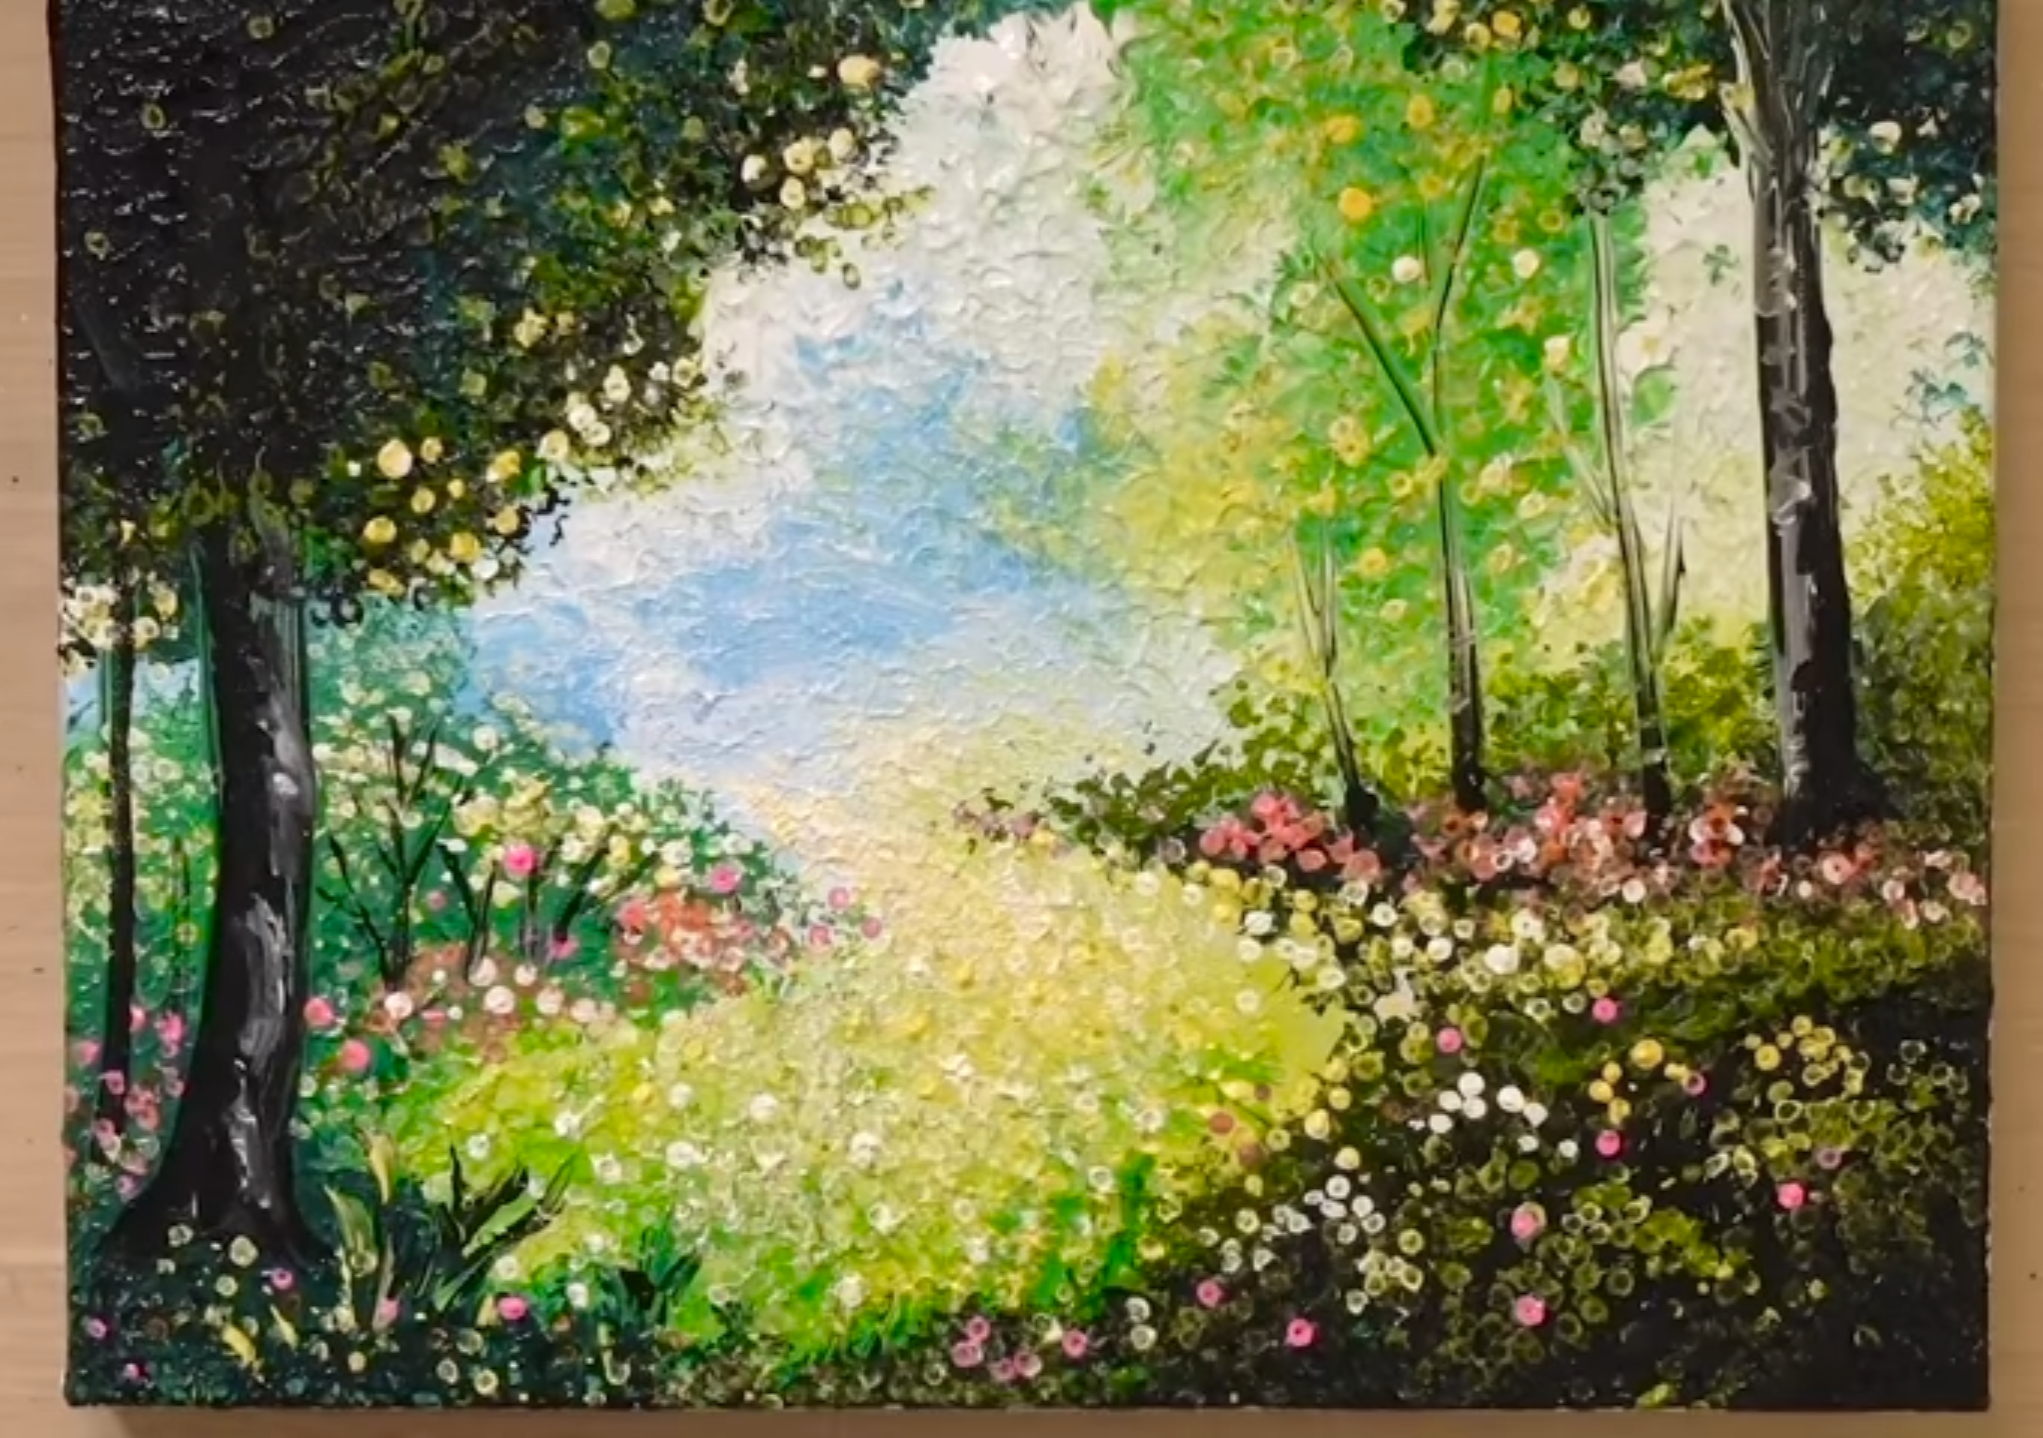
\includegraphics[width=\linewidth]{../images/painting_example_layer_2.png}
                \caption{Детализация объектов на заднем палане}\label{fig:layer2}
            \endminipage\hfill

            \minipage{0.22\textwidth}
                \includegraphics[width=\linewidth]{../images/painting_example_layer_3.png}
                \caption{Основные объекты}\label{fig:layer3}
            \endminipage\hfill

            \label{fig:figure}
        \end{figure}

                Поэтому стоит попробовать сначала заполнять картинку толстыми, грубыми мазками
                (то есть просто с большей шириной, а в реальной жизни это будет отражаться в большем размере кисти и в более сильном нажатии).
        \item …
    \end{itemize}

\end{document}